\newpage
\section{Praxis} \label{sec:Praxis}
\subsection{Erstellung eines domänenspezifischen NER Modells}\label{sec:ErstellungNerModell}
Wie im Kapitel \ref{sec:NER} erläutert, lässt sich zwischen allgemeinen und domänenspezifischen \ac{NER}-Modellen unterscheiden.\footcite[vgl.][S.47]{nouvel2016} Domänenspezifische Modelle sind dabei solche, die für einen dedizierten Themenbereich erstellt wurden und daher in diesem Kontext besonders gute Ergebnisse erzielen.
Es gibt bereits spezialisierte Modelle im Bereich der Medizin die mit einem medizinischen Korpus trainiert wurden. Dazu zählen zum Beispiel BioBERT, ScispaCy oder Y\footcite[S.12]{li2020}. Diese beinhalten bereits zahlreiche medizinische Konzepte und Entitäten, allerdings mussten wir feststellen, dass auch sie für unseren Anwendungsfall \textit{out of the box} nicht alle erforderlichen Entitäten der hier betrachteten Domäne erkennen. Daher haben wir uns entschlossen ein eigenes Modell für das Themengebiet der Urtikaria-Forschung auf Basis eines sciSpacy Modells zu erstellen.
\subsubsection{Labeling von Trainingsdaten}\label{sec:Labeling}
Das Annotieren von Trainingsdaten hat einen zentralen Anteil bei der Erstellung eines eigenen Modells. Akkurate Daten sind essentiell für die Genauigkeit des resultierenden Modells. Neben der Menge der zum Training zur Verfügung stehenden Daten ist es unterlässlich, dass diese widerspruchsfrei sind.

\subsubsection{Auswahl der Labels}\label{sec:AuswahlLabels}
Die Auswahl der Labels muss für den Anwendungsfall angemessen sein. Je nachdem was die Zielstellung des Projektes ist, können unterschiedliche Labels erforderlich sein, um die notwendigen Zusammenhänge abzubilden.
In der vorliegenden Arbeit wurden 5 Entitäten ausgewählt. Diese sind Disease, Treatment, Biomarker, Diagnostic und Person. Die hier getroffene Auswahl basiert zum einen auf in der einschlägigen Literatur gewählten Labels und zum anderem auf den im Rahmen des CAPTUM Projektes umrissenen Entitäten.\footcite[vgl.][S.]{li2016}\footcite[vgl.][S.]{eickhoff2020}

% \subsubsection{Annotierungsaufgaben}

\subsubsection{Richtlinien zur Annotation}\label{sec:Richtlinien}
Um möglichst homogene, gleichmäßige Annotationen über mehrere Personen hinweg zu erhalten ist es sinnvoll Richtlinien für die Annotation festzulegen. Dies ist häufig ein iterativer Prozess, da zu Beginn einer solchen Aufgabe nicht immer vorab klar ist, an welchen Stellen Unklarheit besteht.[Citation]

Auch wir haben Richtlinien aufgestellt, die sich zum einen mit den von uns gewählten Entitäten selber und zum anderen mit der Art und Weise der Annotation beschäftigen. Die begrifflichen Definitionen sind vor allem vor dem Hintergrund wichtig, dass die beteiligten Personen keinen medizinischen Hintergrund haben und auf diese Art und Weise zunächst ein gemeinsames Grundverständnis davon geschaffen werden soll, was zum Beispiel einen \textit{Biomarker} oder \textit{Diagnostik} ausmacht. An diesem Beispiel wird auch deutlich, dass Entitäten nicht immer trennscharf sind. Biomarker wird demnach definiert als \glqq{}ein messbarer Indikator für das Vorhandensein oder die Schwere eines Krankheitszustands oder eines anderen physiologischen Zustands eines Organismus.\grqq{}\footcite[vgl.]{wiki2021}, medizinische Diagnose als \glqq{}process of determining which disease or condition explains a person's symptoms and signs.\grqq{} Diagnose wird als Prozess des Nachweises einer Krankheit verstanden und Biomarker als Gegenstand des Nachweises. In diesem Falle ist nicht immer einfach zu unterscheiden ob es im vorliegenden Satz um das Vorhandensein eines Stoffes/eines Markers nun im diagnostischem Sinne zu verstehen ist, oder als Marker gekennzeichnet werden sollte.
\footcite[vgl.][]{neves2014}

\subsubsection{Verwendete Software}\label{sec:Software}
Für die Annotation der Entitäten wurde Doccano verwendet.\footcite[vgl.][S.]{hirokinakayama2021} Dabei handelt es sich um ein open source Tool zur Text Klassifikation, Sequenzlabeling und Sequenz zu Sequenz Aufgaben.
Zur Unterstützung der Annotierung und um den Aufwand zu reduzieren, wurde auf das Auto Labeling Feature der Software zurückgegriffen. Dabei kann eine Backendanwendung konfiguriert werden, die auf Basis eines trainierten Modells Vorschläge zur Annotation unterbreitet.
Für diese Funktionalität wurden von uns zunächst die ersten 100 Textabschnitte ohne Backend annotiert und die gewonnenen Daten dann für das initiale Modell verwendet.
\footcite[vgl.][]{neves2014a}

\subsubsection{Analyse zum Inter-Annotator Agreement}\label{sec:Iaa}
Das \acf*{IAA} ist ein Maß der Übereinstimmung von Annotationen die von mehreren Personen getätigt wurden. Von dem Score lassen sich allgemein Rückschlüsse ziehen, wie zuverlässig der Annotierungsprozess ablief. \footcite[vgl.][S.298]{ide2017} Der Grundgedanke dabei ist, dass ein hoher Score für die Reproduzierbarkeit der Ergebnisse spricht und Ausdruck ist von der Klarheit der Richtlinien.

% https://towardsdatascience.com/inter-annotator-agreement-2f46c6d37bf3
\begin{itemize}
    \item Cohens K\footcite[vgl.][S.]{cohen1960}
    \item Fleiss K\footcite[vgl.][S.]{fleiss1971}
\end{itemize}

\subsubsection{Labeling von Trainingsdaten}\label{sec:Labeling}
Das Labeling der Daten wurde von zwei Personen ohne medizinischen Hintergrund ausgeführt. Um dennoch eine möglichst hohe Qualität der Annotationen zu erhalten, haben die teilnehmenden Personen bei Unklarheit im Internet recherchiert. Wie im Abschnitt \ref{sec:IAA} beschrieben ist, wurde dadurch dennoch eine verhältnismäßig gute Genauigkeit erzielt.
Insgesamt wurden dadurch X Textabschnitte annotiert, die zufällig aus dem Gesamtcorpus von 465 einzigartigen Texten ausgewählt wurden. Dies entspricht einem Anteil von circa 0.01\%, relativ gesehen zu der Gesamtzahl von 57764 Abschnitten.

% Das annotieren von Trainingsdaten hat einen zentralen Anteil bei der Erstellung eines eigenen Modells. Akkurate Daten sind essentiell für die Genauigkeit des resultierenden Modells. Neben der Menge der zum Training zur Verfügung stehenden Daten ist es außerdem unerlässlich, dass diese widerspruchsfrei sind.

\begin{itemize}
    \item Notwendige Menge an Annotationen
    \item Aufstellung der Label (Ontologie?)
    \item Richtlininien zur Annotation
    \item Auswahl der Software (Doccano, Spacy)
\end{itemize}
\subsubsection{Training des Modells}\label{sec:ModelTraining}
Für das Training des Modells werden die annotierten Daten aus den vorherigen Schritten verwendet.
Für das Training des Modells wurde die \acl{NLP} Bibliothek spaCy\footcite[]{spacy2} verwendet. Diese wurde im Hinblick auf ihre umfangreichen Funktionalitäten und benutzerfreundlichkeit ausgewählt.

Das Training erfolgt über den \textit{spacy train} Befehl mit Trainingsparametern die über ein config file definiert werden. Die Parameter für das Training des Modells wurden von uns nicht verändert und orientieren sich somit an den empfohlenen Werten.\footcite[vgl.]{ostkamp2021}%\footcite[vgl.]{zotero-193}

Für einige \ac{NLP} tasks wie die \textit{text classification} können unterschiedliche Architekturen gewählt werden, für die \acl{NER} ist nur der \textit{Transition Based Parser} verfügbar.%\footcite{zotero-182}

\begin{itemize}
    \item Warum SpaCy
    \item Modellarchitektur
    %https://spacy.io/api/architectures#TransitionBasedParser
    \item Trainingsparameter
\end{itemize}

% \footcite{zotero-182}
Bei der zugrundeliegenden Architektur handelt es sich um einen sogenannten Transition Based Parser. Diesem liegt das Konzept von Übergängen zwischen Wörtern zugrunde. Auf Basis der Annahme, dass der \acl{POS} tag eines Wortes abhängig ist von bisherigen Wörtern (dem sogenannten \textit{state}) eines Satzes, lassen sich Wahrscheinlichkeiten für Übergänge vom letzten hin zum nächsten Tag aufstellen.\footcite{honnibal2013a} Diese werden in eine sogenannte \textit{transition matrix} überführt, die die Wahrscheinlichkeiten enthält für die Nachfolge eines Tags auf einen anderen.
% \begin{itemize}
%     \item Spacy CLI
%     \item Training mit default settings
% \end{itemize}

Wie im Kapitel \ref{sec:NER} beschrieben, werden zur Evaluierung eines Modells der f-Score verwendet, der aus XY berechnet wird. Dieser setzt sich aus Precision und Recall, also dem Anteil der XY zusammen.

\begin{figure}[H]
    \centering
    \caption[]{Precision, Recall und Score}
	\label{fig:TrainPrecisionRecall}
    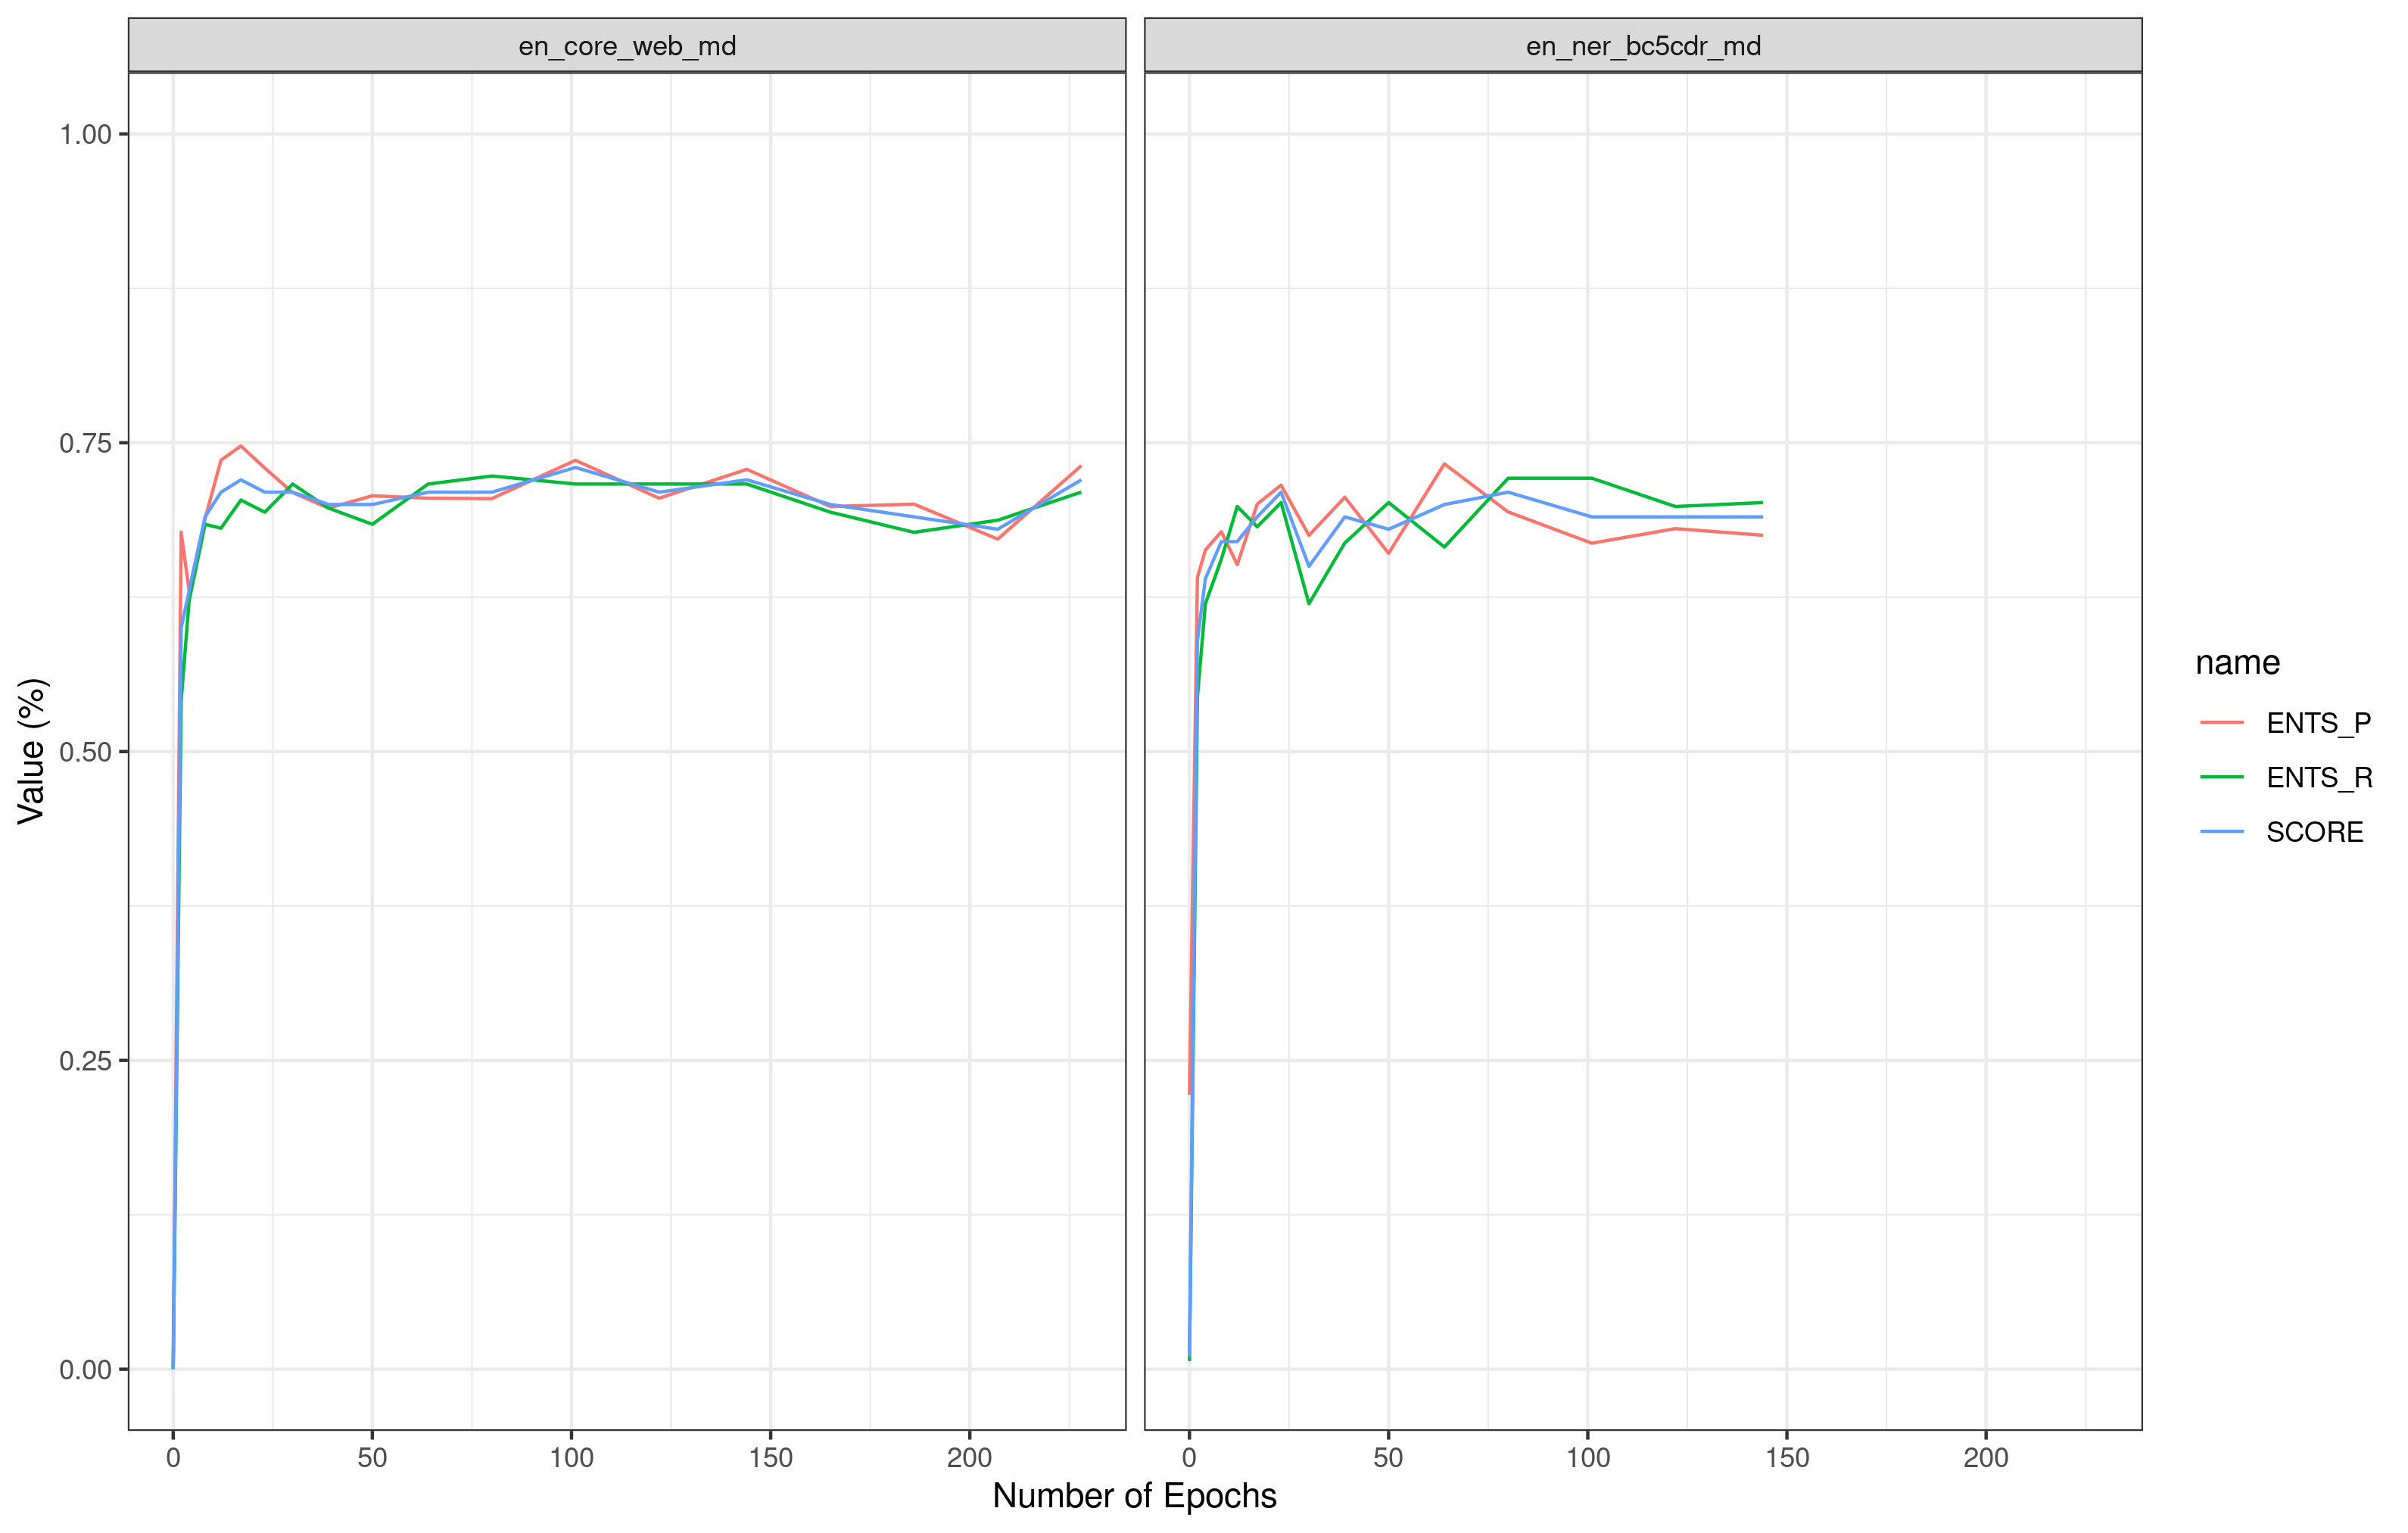
\includegraphics[width=1\textwidth]{spacy_train_precision_recall}
\end{figure}
In Abbildung \ref{fig:TrainPrecisionRecall} sind Precision, Recall und der f-Score des Trainings für zwei Basismodelle dargestellt. Diese sind das spaCy-eigene \glqq{en\_core\_web\_md}\grqq{} und das im Rahmen der BioCreative 5 Challenge erstellte \glqq{en\_ner\_bc5cdr\_md}\grqq. Für beide Modelle gilt, dass sich das Verhältnis von Precision und Recall über mehrere Trainingsepochen hinweg nicht wesentlich verbessert beziehungsweise stagnativ bei circa 70\% einpendelt. Die Wahl des Modells macht unter dieser Betrachtung folglich nicht wesentlich einen Unterschied. Dies deutet darauf hin, dass das Modell beim Training nicht wesentlich konvergiert, das heißt in XY übergeht.

Die Wahl des Basismodells für das weitere Annotieren sowie nachfolgende Schritte fiel dennoch auf das scispacy Modell, da dieses insgesamt mit mehr Daten trainiert wurde. Daher gehen wir davon aus, dass dieses Modell besser generalisieren wird, das heißt bei unbekannten Daten bessere Klassifikationen treffen wird.
% \footcite[vgl.]{zotero-163}\footcite[vgl.]{zotero-165}
\begin{figure}[H]
    \centering
    \caption[]{Verluste (\textit{losses}) bei \ac{NER} und TOK2VEC}
	\label{fig:TrainLosses}
    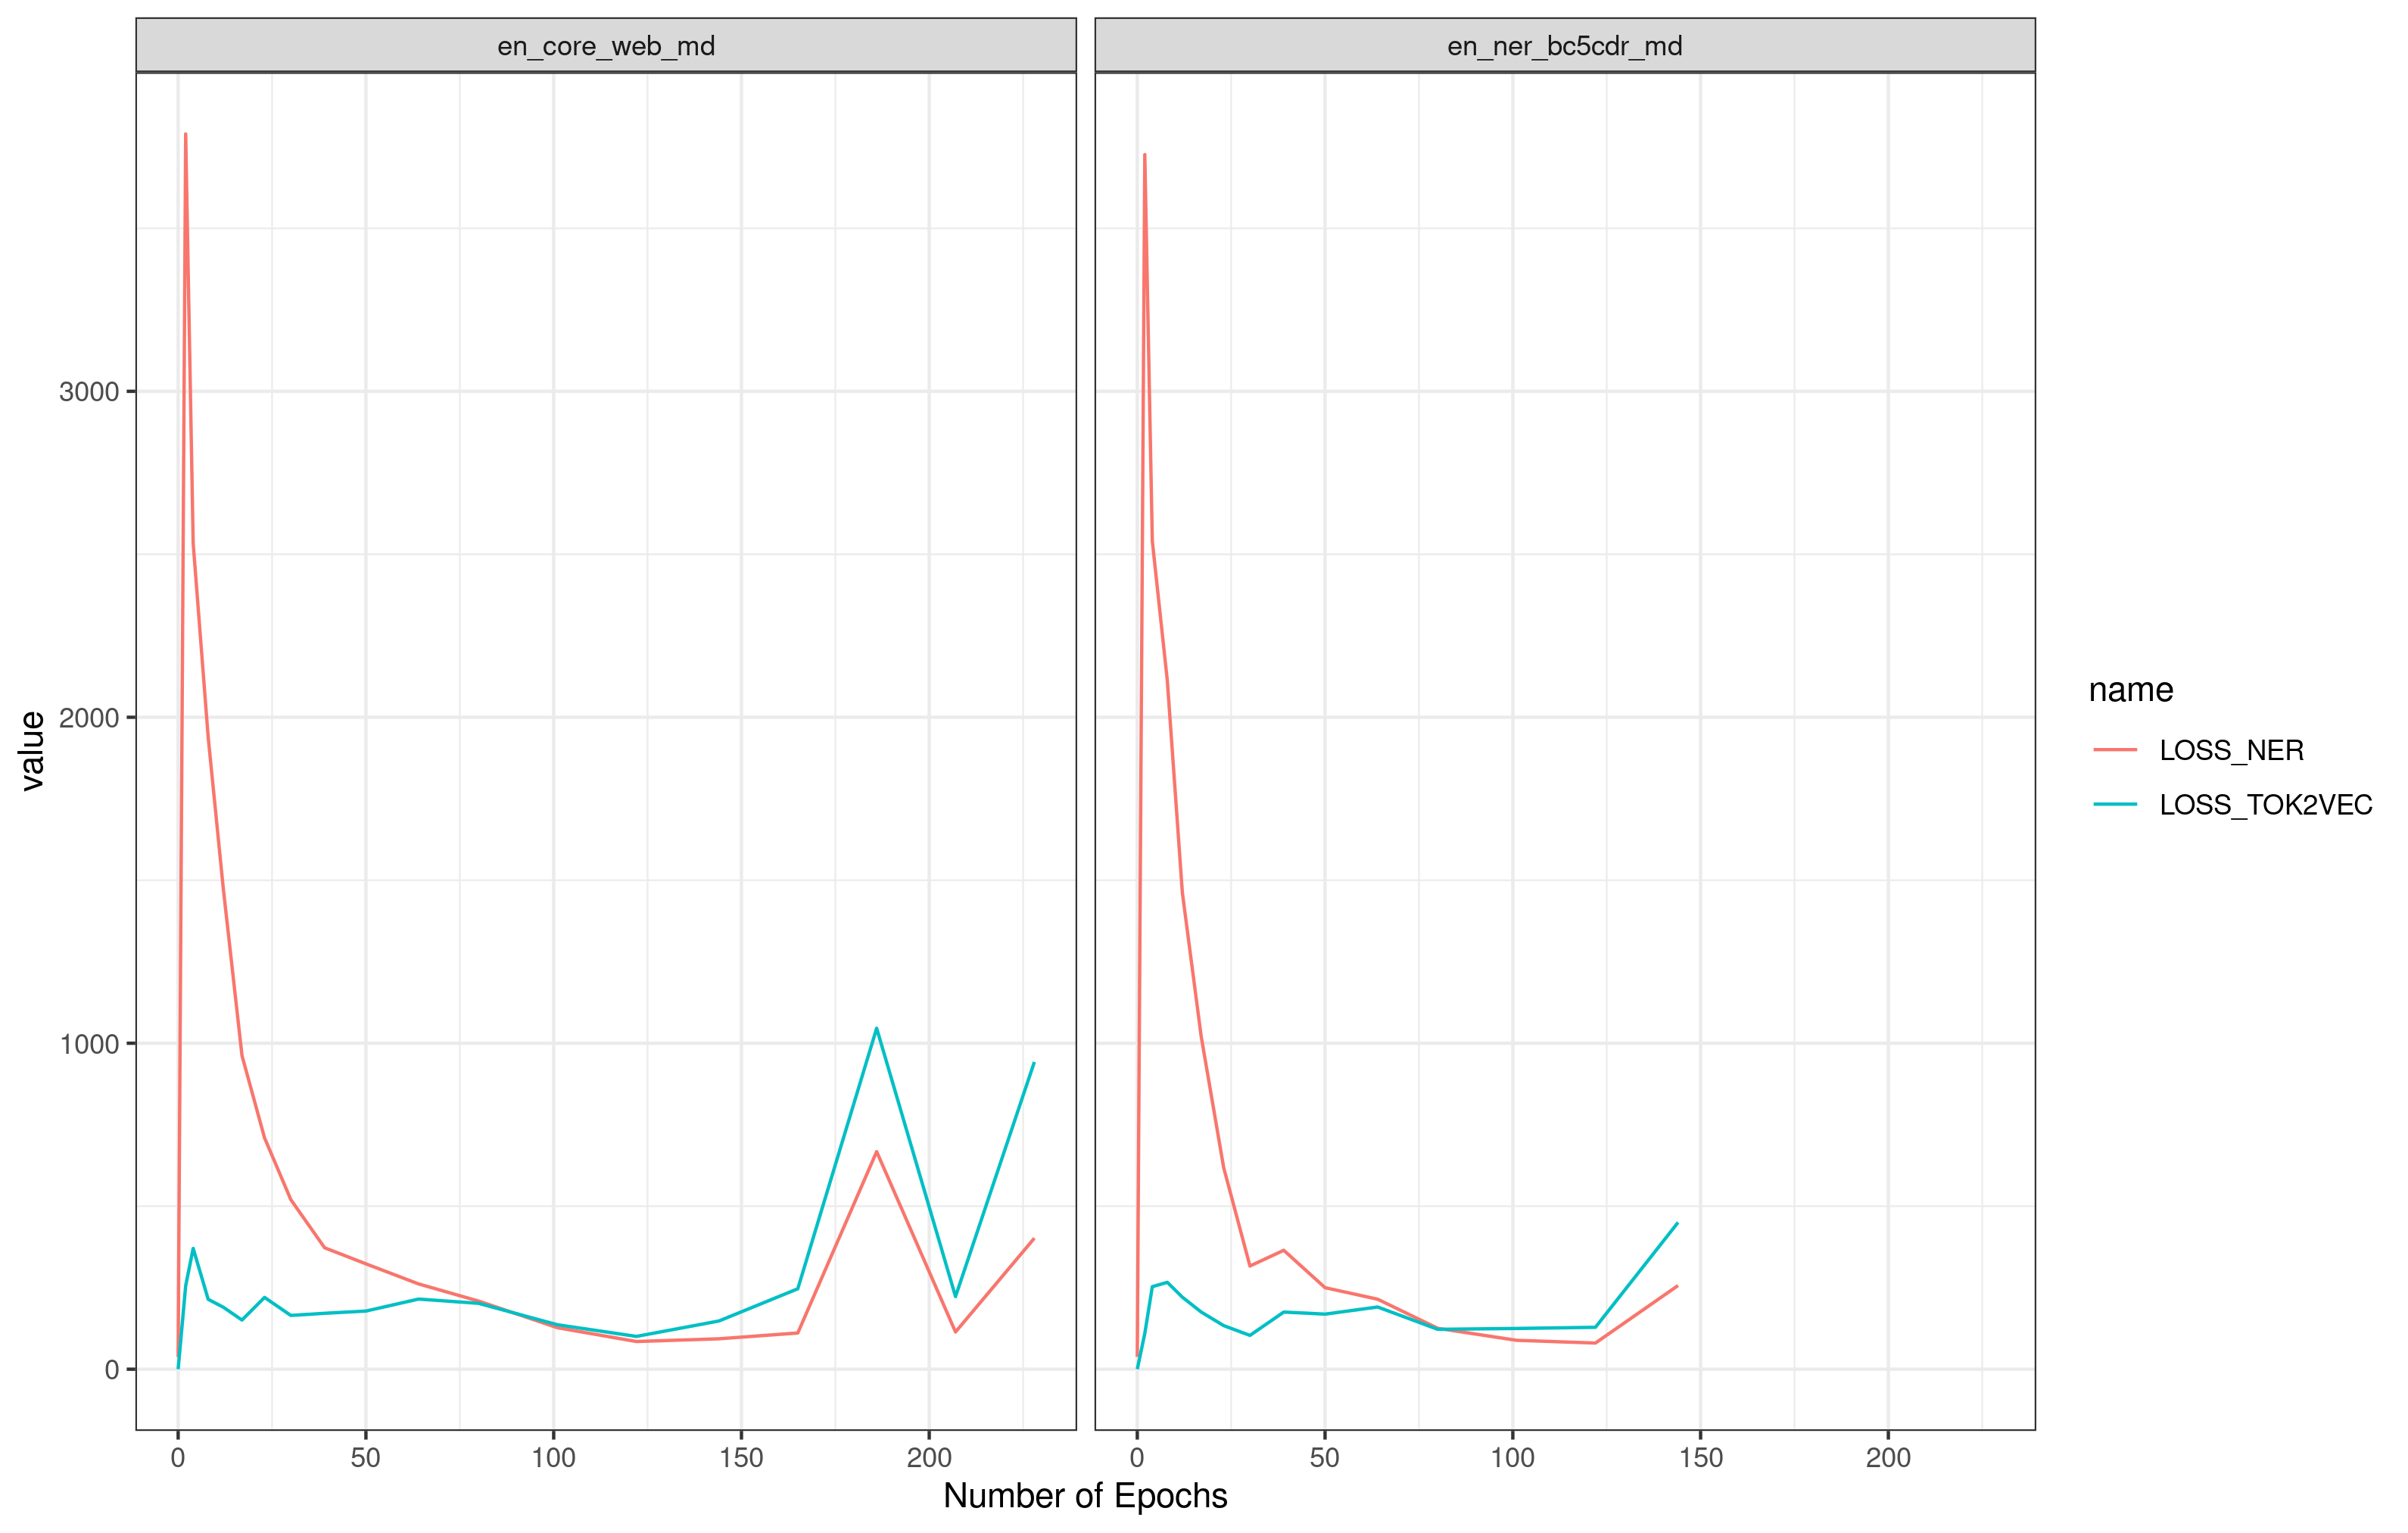
\includegraphics[width=1\textwidth]{spacy_train_losses}
\end{figure}
\footcite[]{tsai2006}

Was sind Verluste??

Zum weiteren Verständnis des Modells und der Vorhersagen, ist es sinnvoll, dieses feiner zu analysieren. So kann die Genauigkeit des Modells weiter für jede Entität aufgeschlüsselt werden.

\begin{figure}[H]
    \centering
    \caption[]{F-Score je Entität}
	\label{fig:TrainEntities}
    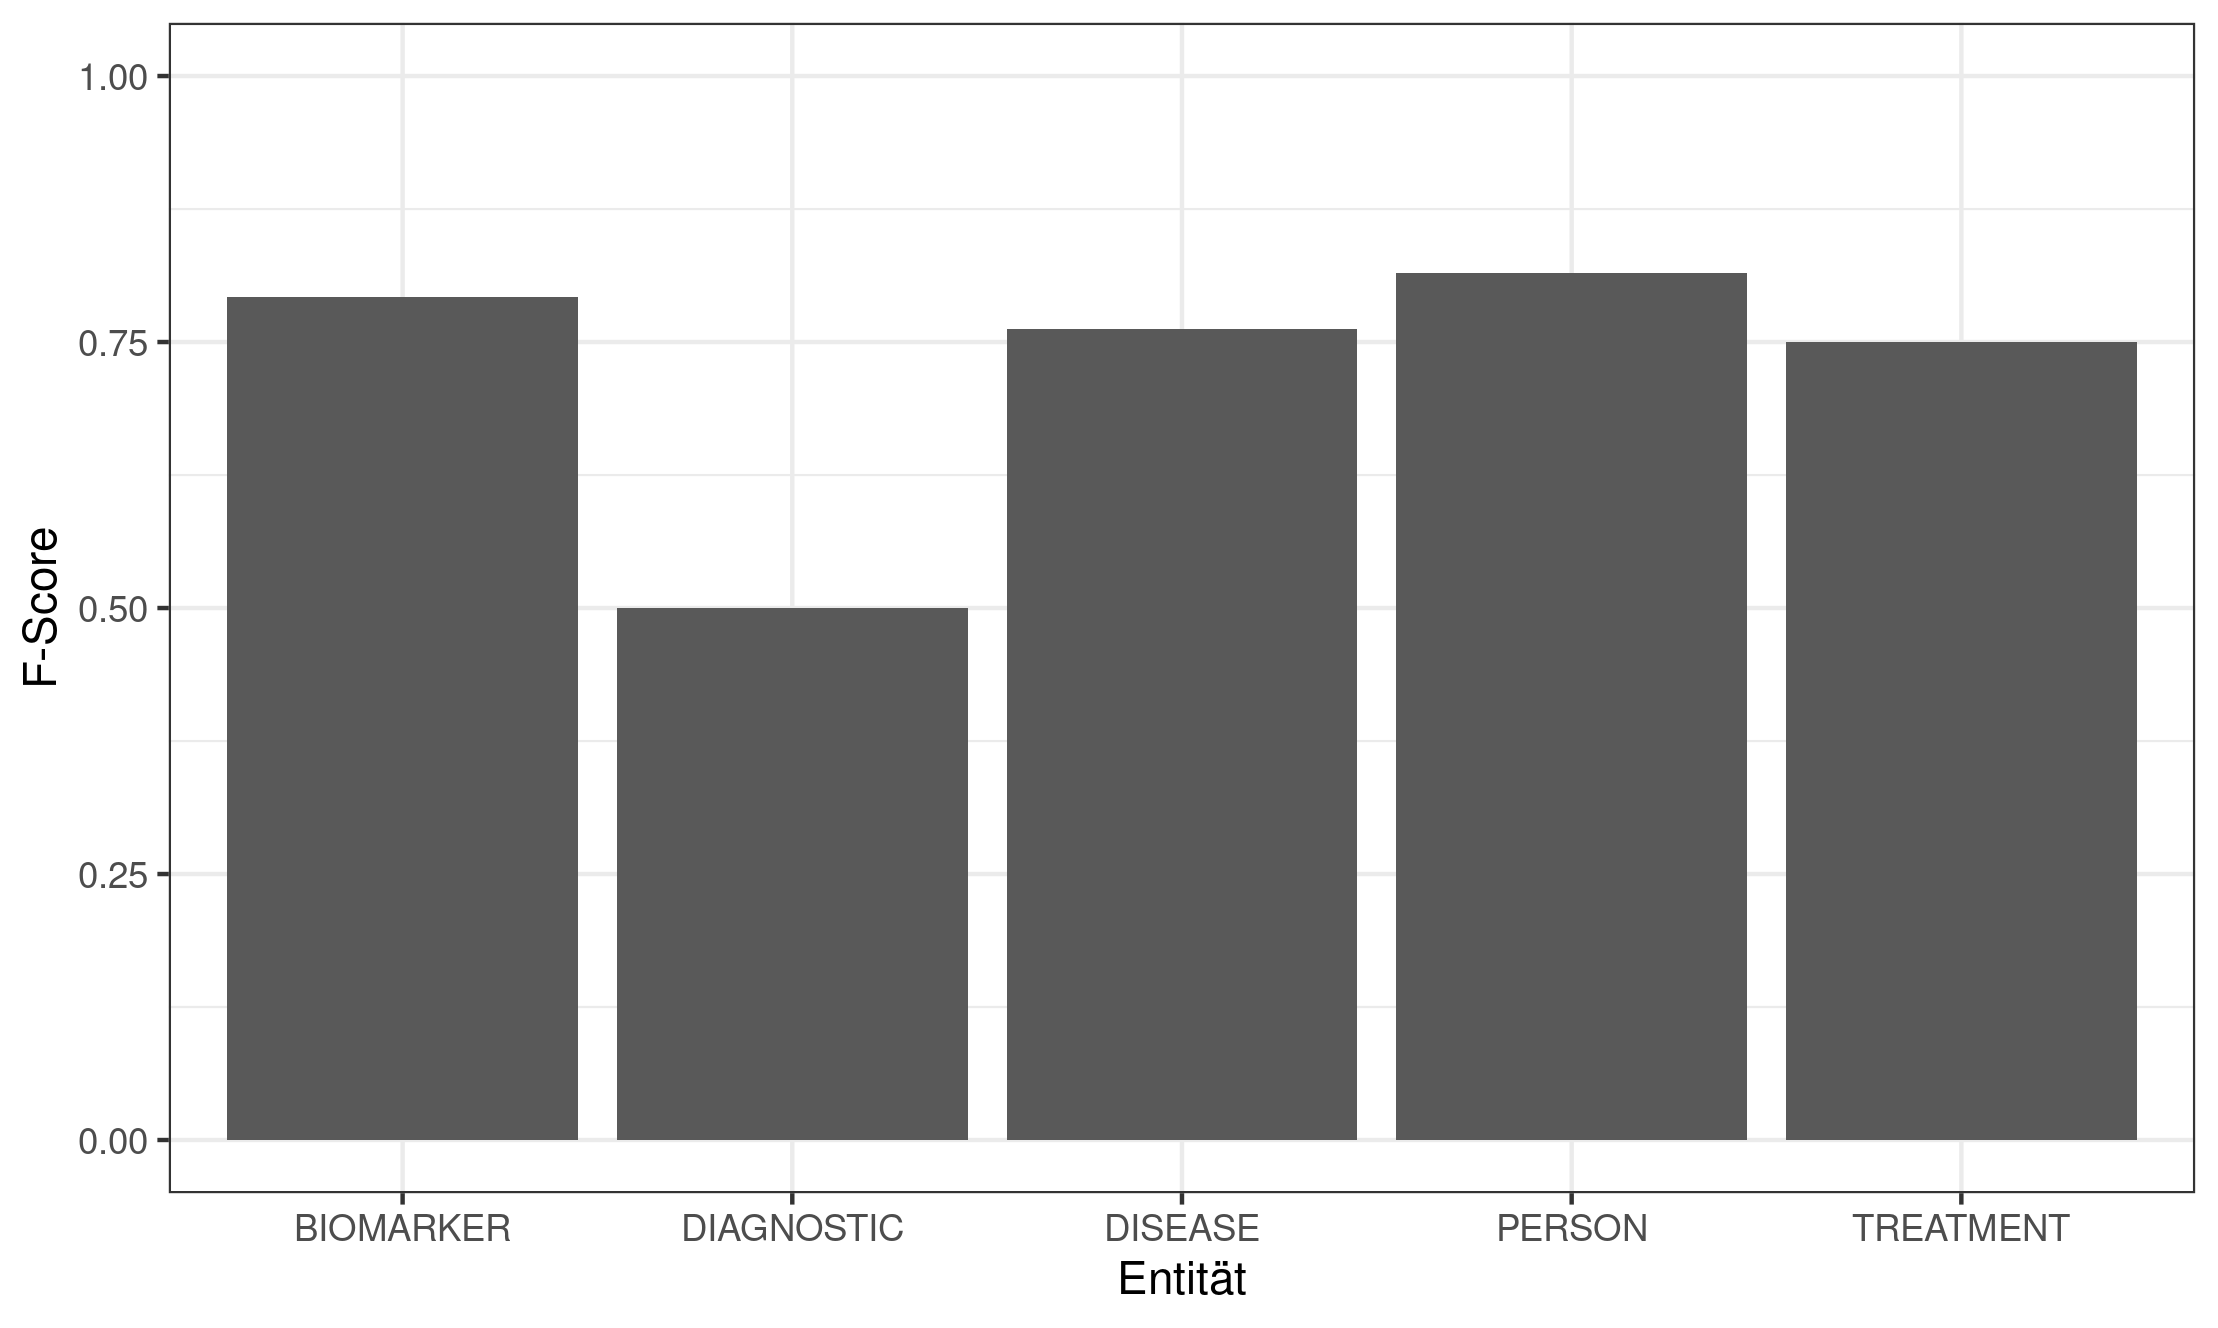
\includegraphics[width=1\textwidth]{spacy_train_entities}
\end{figure}
Abbildung \ref{fig:TrainEntities} stellt den F-Score je Entität dar. Es ist erkennbar, dass die Entitäten Biomarker, Disease, Person und Treatment einen sehr homogenen Score haben, Diagnostic jedoch deutlich darunter liegt. Ursächlich hierfür könnte die relativ geringe Anzahl an Trainingsdaten für das Diagnostic Label sein. Insgesamt liegt die Anzahl bei X, währenddessen bei den anderen Labels jeweils mindestens Y Textsamples vorhanden sind. Zur weiteren Verbesserung des F-Scores und somit des Modells, sollten folglich mehr Annotationen mit dem Diagnostic Label gesammelt werden.

% \subsection{Markeranalyse}
% \subsection{Überführung in Tabellenstruktur}
% \subsection{Markerkorrelationen}
% \subsection{Aufstellung des Gradingsystems}
